\newpage
{\bfseries ҒТАМР 20.53.19}
\hfill {\bfseries \href{https://doi.org/10.58805/kazutb.v.3.24-423}{https://doi.org/10.58805/kazutb.v.3.24-423}}

\sectionwithauthors{ Ж.С. Есенгалиева, Ж.О. Оралбекова, М.К.Турарова}{МЕДИЦИНА САЛАСЫНДА КОМПЬЮТЕРЛІК КӨРУ ӘДІСТЕРІНІҢ НЕГІЗІНДЕ ГРАФИКАЛЫҚ АҚПАРАТТЫ ӨҢДЕУ}

\begin{center}
 
{\bfseries Ж.С.~Есенгалиева\textsuperscript{🖂}, Ж.О. Оралбекова, М.К.
Турарова}

Л.Н.~Гумилев атындағы Еуразия ұлттық университеті, Астана, Қазақстан,
\end{center}
Корреспондент-автор: \emph{jannayess@gmail.com} \vspace{0.5cm}

Мақалада медициналық бейнелерді талдауда қолданылатын сегменттеу
әдістері сипатталған. Маг-ниттік резонансты томография және компьютерлік
томография кескіндерін талдауда қолданылатын шекті мәндер,
классификация, кластерлеу, Марков желілері, нейрондық желілер,
деформациялана-тын модельдер сияқты әдістердің артықшылықтары мен
кемшіліктері қарастырылады. Денсаулық сақтау саласында компьютерлік
көруді пайдалана отырып, графикалық деректерді өңдеуге арналған
бағдар-ламалық қамтамасыз ету технологиясын әзірлеу процесі ұсынылған.
Әзірленген жүйені жоба-лау және модельдеу кезеңдері сипатталған. Кескінді
сегменттеу арқылы деректерді өңдеу диагности-калық дәлдікке және қолданба
пайдаланушылары арасындағы тығыз өзара әрекеттесуге ықпал етеді.
Сондай-ақ, қолданбалар бұлтында зерттеу көлемін сақтауға мүмкіндік
беретін дерекқор және кросс-платформалық қосымша жасалды. Құрылған
мобильді қосымшаны толық тестілеу жүргізілді. Ден-саулық сақтау саласында
медициналық кескінді сегменттеу дәлірек диагноз қою және пациенттің
диагнозын одан әрі тексеру үшін барған сайын қажетті функцияға айналуда.
Сондықтан түрлі ауру-ларды дер кезінде анықтаудың арқасында ол неғұрлым
ұтымды әрі мақсатты емделуде, халықтың өмір сүру сапасын жақсартуда
кеңінен пайдаланылмақ. Қолданбаны әзірлеу кезінде графикалық деректерді
талдауды жеңілдететін Open CV, Tensorflow, PyTorch кітапханаларды
қолдану арқылы деректерді өңдеу жүргізілді.

{\bfseries Түйін сөздер:} компьютерлік көру, OpenCV, Tensorflow,
сегментация, графикалық деректерді өңдеу.


\sectionheading{ОБРАБОТКА ГРАФИЧЕСКИХ ДАННЫХ НА ОСНОВЕ МЕТОДОВ КОМПЬЮТЕРНОГО ЗРЕНИЯ В СФЕРЕ МЕДИЦИНЫ}
\begin{center}


{\bfseries Ж.С.~Есенгалиева\textsuperscript{🖂}, Ж.О. Оралбекова,
М.К.~Турарова}

Евразийский национальный университет имени Л.Н.~Гумилева, Астана,
Казахстан,

e-mail: jannayess@gmail.com
\end{center}

В статье описаны методы сегментации, используемые при анализе
медицинских изображений. Рассмотрены преимущества и недостатки таких
методов как пороговые значения, классификация, кластеризация, Марковские
сети, нейронные сети, деформируемые модели, используемых при ана-лизе
изображений магнитно-резонансной томографии и компьютерной томографии.
Представлен процесс разработки программной технологии обработки
графических данных с использованием ком-пьютерного зрения в сфере
здравоохранения. Описаны этапы проектирования и моделирования
разработанной системы. Обработка данных посредством сегментации
изображений способствует точности диагностирования и тесного
взаимодействия между пользователями приложения. Также создана база
данных и кроссплатформенное приложение, позволяющее хранить объем
исследований в облаке приложений. Проведено полное тестирование
созданного мобильного приложения. В сфере здравоохранения сегментация
медицинских изображений становится все наиболее необходимой \\функцией для
более точной диагностики и дальнейшей верификации диагноза пациента, а
потому, благодаря своевременному выявлению различных заболеваний, будет
широко использоваться для более рационального и целенаправленного
лечения, улучшающее качество жизни населения. При разработке приложения
обработка данных осуществлялась с помощью таких библиотек, как OpenCV,
Tensorflow, PyTorch, которые способствуют анализу графических данных.

{\bfseries Ключевые слова:} компьютерное зрение, OpenCV, Tensorflow,
сегментация, обработка графичес-ких данных.


\sectionheading{PROCESSING OF GRAPHIC DATA BASED ON COMPUTER VISION METHODS IN THE FIELD OF MEDICINE}
\begin{center}
{\bfseries Zh.S. Yessengaliyeva\textsuperscript{🖂}, Zh.O. Oralbekova, M.K.
Turarova}

L.N. Gumilyov Eurasian national university, Astana, Kazakhstan,

e-mail: jannayess@gmail.com
\end{center}

The article describes segmentation methods used in the analysis of
medical images. The advantages and disadvantages of such methods as
threshold values, classification, clustering, Markov networks, neural
networks, deformable models used in the analysis of magnetic resonance
imaging and computed tomography images are considered. The process of
developing software technology for processing graphic data using
computer vision in the healthcare sector is presented. The stages of
design and modeling of the developed system are described. Data
processing through image segmentation promotes diagnostic accuracy and
close interaction between application users. A database and
cross-platform application have also been created that allows you to
store a volume of research in the application cloud. Full testing of the
created mobile application was carried out. In the healthcare sector,
medical image segmentation is becoming an increasingly necessary
function for more accurate diagnosis and further verification of the
patient's diagnosis, and therefore, thanks to the timely detection of
various diseases, it will be widely used for more rational and targeted
treatment, improving the quality of life of the population. When
developing the application, data processing was carried out using
libraries such as OpenCV, Tensorflow, PyTorch, which facilitate the
analysis of graphical data.

{\bfseries Keywords:} computer vision, OpenCV, Tensorflow, segmentation,
processing of graphic data.
\begin{multicols}{2}

{\bfseries Кіріспе.} Компьютерлік көру айналасындағы заттарды қабылдауға,
жіктеуге, тануға және жауап беруге мүмкіндік береді. Медициналық
кескінді өңдеу, іздеу мен талдауды жеңілдету үшін өңделмеген кескіндерді
өлшенетін символдық пішінге түрлендіру, диагностикаға көмектесу үшін
мәнді сандық ақпаратты алу және көптеген кескіндеу әдістерінен қосымша
деректерді біріктіру үшін пайдалы. Медициналық кескінді талдаудың іргелі
мәселелерінің бірі кескіндердегі органдар немесе қалыптан тыс аймақтар
(мысалы, ісіктер) сияқты объектілердің шекараларын анықтайтын кескін
сегментациясы болып табылады. Сегменттеу нәтижесінің болуы пішінді
талдауға, көлемнің өзгеруін анықтауға және дәл сәулелік терапия
жоспарына мүмкіндік береді.

Жақында медициналық кескіндерді сегмента-циялау әдебиетінде бірнеше жалпы
әдістер пайда болды {[}1{]}. Сегменттеу әдістерін келесі санатқа
бөлеміз: шекті мән тәсілдері, аймақты кеңейту тәсілдері, жіктеуіштер,
кластерлеу тәсілдері, Марковтың кездейсоқ өріс модельдері (MRF), жасанды
нейрондық желілер, деформацияланатын модельдер, атласқа негізделген
тәсілдер.

Шекті мән скалярлық кескіндерді кескін қарқындылығының екілік бөлінуін
жасау арқылы бөлуге жақындайды. Шекті белгілеу процедурасы қажетті
сыныптарды бөлетін шекті деп аталатын қарқындылық мәнін анықтауға
тырысады. Содан кейін сегментацияға барлық пикселдерді шекті мәннен
асатын бір сыныпқа, ал қалған пикселдерді басқа сыныпқа топтастыру
арқылы қол жеткізіледі. Бірнеше шекті мәнді анықтау -- бұл бірнеше шекті
деп аталатын процесс. Шекті мән көбінесе суретті өңдеудің реттілігінде
бастапқы қадам ретінде қолданылады. Сонымен қатар, шекті мән әдетте
кескіннің кеңістіктік сипаттамаларын ескермейді. Бұл оны
магниттік-резонанстық бейнелерде пайда болатын шу мен қарқындылықтың
гетерогенділігіне сезімтал етеді.

Аймақты кеңейту тәсілдері -- бұл алдын ала анықталған критерийлерге
негізделген кескін аймағын алу әдісі. Бұл өлшемдер кескіннің
қарқындылығы немесе жиектері туралы ақпаратқа негізделуі мүмкін.
Қарапайым түрде, ауданды ұлғайту үшін бастапқы нүкте қажет, оны оператор
қолмен таңдайды және кейбір алдын ала анықталған критерийлер негізінде
бастапқы мәнге байланысты барлық пикселдерді алады. Осылайша,
өндірілетін әрбір аймақ үшін алғашқы нүкте алыну керек. Аймақтың ұлғаюы
шуға да сезімтал болуы мүмкін, нәтижесінде алынған аймақтардың тесіктері
болады немесе тіпті ажыратылады {[}2{]}.

Жіктеуіштер әдістері - белгілі белгілері бар деректерді қолдана отырып,
кескіннен алынған объектілердің кеңістігін бөлуге тырысатын үлгіні тану
әдістері. Нысандар кеңістігі -- бұл кез-келген кескін функциясының
ауқымы, ал объектілердің ең көп таралған кеңістігі -- кескіннің
қарқындылығы. Жіктеуіштер -- бақылау әдістері деп аталады, өйткені олар
оқу деректерін қолмен сегментациялауды қажет етеді және оны жаңа
деректерді автоматты түрде сегментациялау үшін критерий ретінде
пайдаланады. Ең қарапайым жіктеуіштер -- бұл ең жақын көршінің
классификаторы {[}3{]}, онда әр пиксель жақын қарқындылықтағы жаттығу
мәліметтерімен бірдей сыныпта жіктеледі. Тағы бір параметрлік емес
классификатор -- Parzen терезелері, онда жіктеу таңбаланған пиксельдің
қарқындылығына негізделген объектілер кеңістігінің алдын ала анықталған
терезесінде өлшенген шешім қабылдау процесі арқылы жүзеге асырылады.
Стандартты жіктеуіштер сегменттелген құрылымдардың әртүрлі сандық
сипаттамаларға ие болуын талап етеді.

Кластерлеу алгоритмдері оқу деректерін пайдаланбай, классификатор
әдістерімен бірдей функцияны орындайды. Сондықтан оларды бақыланбайтын
әдістер деп атайды. Оқу деректерінің жетіспеушілігін өтеу үшін
кластерлеу әдістері кескінді сегментациялау {[}4{]} мен әр сыныптың
қасиеттерін сипаттау арасында итеративті түрде ауысады. Әдетте
қолданылатын үш кластерлік алгоритм -- бұл негізгі құралдар немесе
жарияланған алгоритм, анық емес c -- орташа алгоритм және математикалық
күтуді максимизациялау алгоритмі. Кластерлеу алгоритмдері оқыту
деректерін қажет етпесе де, олар бастапқы сегментацияны қажет етеді.
Алайда, кеңістіктік модельдеудің болмауы жылдам есептеу үшін айтарлықтай
артықшылықтар бере алады. Кластерлеу алгоритмдерінің магниттік резонанс
кескіндеріндегі қарқындылықтың гетерогенділігіне тұрақтылығын арттыру
бойынша жұмыс үлкен жетістік көрсетті.

Марковтың кездейсоқ өріс модельдері (MRF) -- бұл жергілікті
корреляциялар кескіннің әртүрлі қасиеттерін модельдеу механизмін ұсынады
{[}5{]}. Медициналық визуализацияда олар әдетте қолданылады, өйткені
пикселдердің көпшілігі көрші пикселдермен бірдей сыныпқа жатады.
Физикалық тұрғыдан алғанда, бұл тек бір пиксельден тұратын кез-келген
анатомиялық құрылымның MRF болжамында пайда болу ықтималдығы өте төмен
екенін білдіреді. MRF әдістері әдетте үлкен есептеу шығындарын
алгоритмдерді қажет етеді. Осы кемшіліктерге қарамастан, MRF тек
сегменттеу кластарын модельдеу үшін ғана емес, сонымен қатар, сандық
маммограммаларды сегментациялау кезінде пайдалы магниттік-резонанстық
суреттерде және текстуралық қасиеттерде пайда болатын қарқындылықтың
гетерогенділігін модельдеу үшін кеңінен қолданылады.

Жасанды нейрондық желілер (ANNs - Artificial neural network) --
биологиялық оқытуды еліктейтін өңдеу элементтерінің немесе түйіндердің
параллель желілері. Оқыту түйіндер арасындағы қосылыстарға тағайындалған
таразыларды бейімдеу арқылы жүзеге асырылады. Медициналық визуализацияда
жіктеуіш ретінде кеңінен қолданылады, онда салмақ жаттығу деректерін
қолдану арқылы анықталады, содан кейін ANN жаңа деректерді сегменттеу
үшін қолданылады. Жасанды нейрондық желілер денсаулық сақтау саласында
пайдалану бетті тексеру жүйесіне ұқсас. Денсаулық нейрондық желісі екі
кіріс кескіннен тұрады, онда бірінші кескін таргетбокс ішінде, ал
екіншісі үміткер кескін аймағы болып табылады. Шығару ретінде суреттер
арасындағы ұқсастық дәрежесі талданады. Денсаулық сақтау желісінде
барлық үміткерлерге әртүрлі кадрларда барудың қажеті жоқ. Оның орнына
конволюциондық желіні пайдаланамыз және әрбір кескінді тек бір рет
айналдыра аламыз {[}6{]}. Әрине, қазіргі әлемде нейрондық желілер адам
қызметінің барлық салаларында кеңінен қолданылады, мысалы, мәтіндік
деректердің үлкен көлемін өңдеуге байланысты проблемаларды талдайды және
талдаудың тиімділігін арттыру үшін деректерді өңдеудің таратылған
жүйелерін қолдану мүмкіндіктерін талқылайды {[}7{]}.

Деформацияланатын модельдер -- бұл ішкі және сыртқы күштердің әсерінен
деформацияланатын жабық параметрлік қисықтарды немесе беттерді қолдана
отырып, аймақтардың шекараларын анықтайтын физикалық модельдерге
негізделген әдістер. Суреттегі объектінің шекарасын белгілеу үшін
алдымен жабық қисық немесе бетті қалаған шекараның жанына қою керек,
содан кейін оны итеративті релаксация процедурасынан өтуге мүмкіндік
береді. Ішкі күштер деформация кезінде оны тегіс ұстау үшін қисықтың
немесе беттің ішінен есептеледі. Сыртқы күштер әдетте кескіннен қисық
сызықты немесе бетті қажетті қызығушылық объектісіне бағыттау үшін
шығарылады. Деформацияланатын модельдер медициналық кескіндерді
сегментациялауда кеңінен қолданылады. Деформацияланатын модельдер жүрек
кескіндерін, компьютерлік томография кескіндеріндегі сүйектерді және
ультрадыбысты сегментациялауда да қолданылды. Деформацияланатын
модельдердің негізгі артықшылықтары -- олардың кескіндерден жабық
параметрлік қисықтарды немесе беттерді тікелей құру. Кемшілігі -- олар
бастапқы модельді орналастыру және тиісті параметрлерді таңдау үшін
қолмен өзара әрекеттесуді қажет етеді {[}8{]}.

Атласқа негізделген тәсіл стандартты атлас немесе шаблон болған кезде
медициналық кескіндерді сегментациялаудың қуатты құралы болып табылады.
Атлас -- бұл сегментацияны қажет ететін анатомиялық құрылымдар туралы
ақпарат жиынтығы. Содан кейін атлас жаңа суреттерді сегментациялау үшін
анықтамалық негіз ретінде қолданылады. Атласқа негізделген
тұжырымдамалық тәсіл классификаторға ұқсас, бірақ оны объект
кеңістігінде емес, кескіннің кеңістіктік аймағында жүзеге асырумен
сипатталады. Атласқа негізделген тәсіл негізінен мидың МРТ кескіндерінде
әртүрлі құрылымдарды сегментациялау және бас сканерлеу кезінде мидың
көлемін анықтау үшін қолданылды. Атласқа негізделген тәсілдің
артықшылығы -- тегтер сегментация сияқты орнатылады. Ол морфологиялық
сипаттамаларды зерттеудің стандартты жүйесін ұсынады. Атласқа
негізделген тәсілдер зерттелетін популяцияда тұрақты болып табылатын
құрылымдарды сегментациялауға жақсы сәйкес келеді.

Осылайша, компьютерлік көрудің сегменттеу әдістері медицина саласында
анатомияны визуализациялаудың маңызды компоненті болып табылады.

{\bfseries Материалдар мен әдістер.} Зерттеушілер әртүрлі қосымшалар мен
жобаларды компьютер-лік көру мүмкіндіктерімен қамтамасыз ету үшін
көптеген құралдар мен бағдарламалық кітапханаларды ойлап тапты. Зерттеу
барысында сегментация әдісін қамитын OpenCV кітапханасы мен Tensorflow
құрылымын пайдалануды таңдадық.

OpenCV кітапханасының негізгі мақсаты -- өте күрделі қосымшаларда
компьютерлік көру технологиясын қолдануды жеңілдетуге көмектесетін
қарапайым интерфейсті ұсыну. Бұл кітапхана қолдайтын мүмкіндіктер
денсаулық сақтау, қауіпсіздік, стерео көру және робототехника сияқты
компьютерлік көрудің әртүрлі салаларын қамтиды. Сонымен қатар, OpenCV
кітапханасында Maсhing Learning модулі бар {[}3{]}.

TensorFlow міндеттерінің бірі -- терең нейрондық желілерді енгізу және
оқыту немесе суреттерді классификациялау және сегментациялау {[}9{]}.

Медициналық қызмет көрсету саласында компьютерлік көруді пайдалана
отырып, графикалық деректерді өңдеуге арналған бағдарламалық қамтамасыз
ету технологиясын әзірлеу процесінде функционалдың жобалауы жүргізілді.
Солардың ішінде класс, реттілік, күй және пайдалану жағдайларының
диаграммалары құрылды. Әзірленген қосымшада екі негізгі қолданушы түрі
бар: науқас және дәрігер. 1-суретте графикалық деректердің жүру картасы
көрсетілген. Бастапқы деректер, яғни медициналық сурет «науқас»
қолданушы арқылы жүйеге жүктеледі. «Дәрігер» қолданушы функционалдығы
сегментация аймағына ие. Ол сәйкес парақшаға көшіп деректерді, яғни
медициналық суретті сегментацияға арналған модуль арқылы суретті
өңдейді. Өңделген деректер нәтиже құруға мүмкіндік береді.
\end{multicols}

\begin{figure}[H]
	\centering
	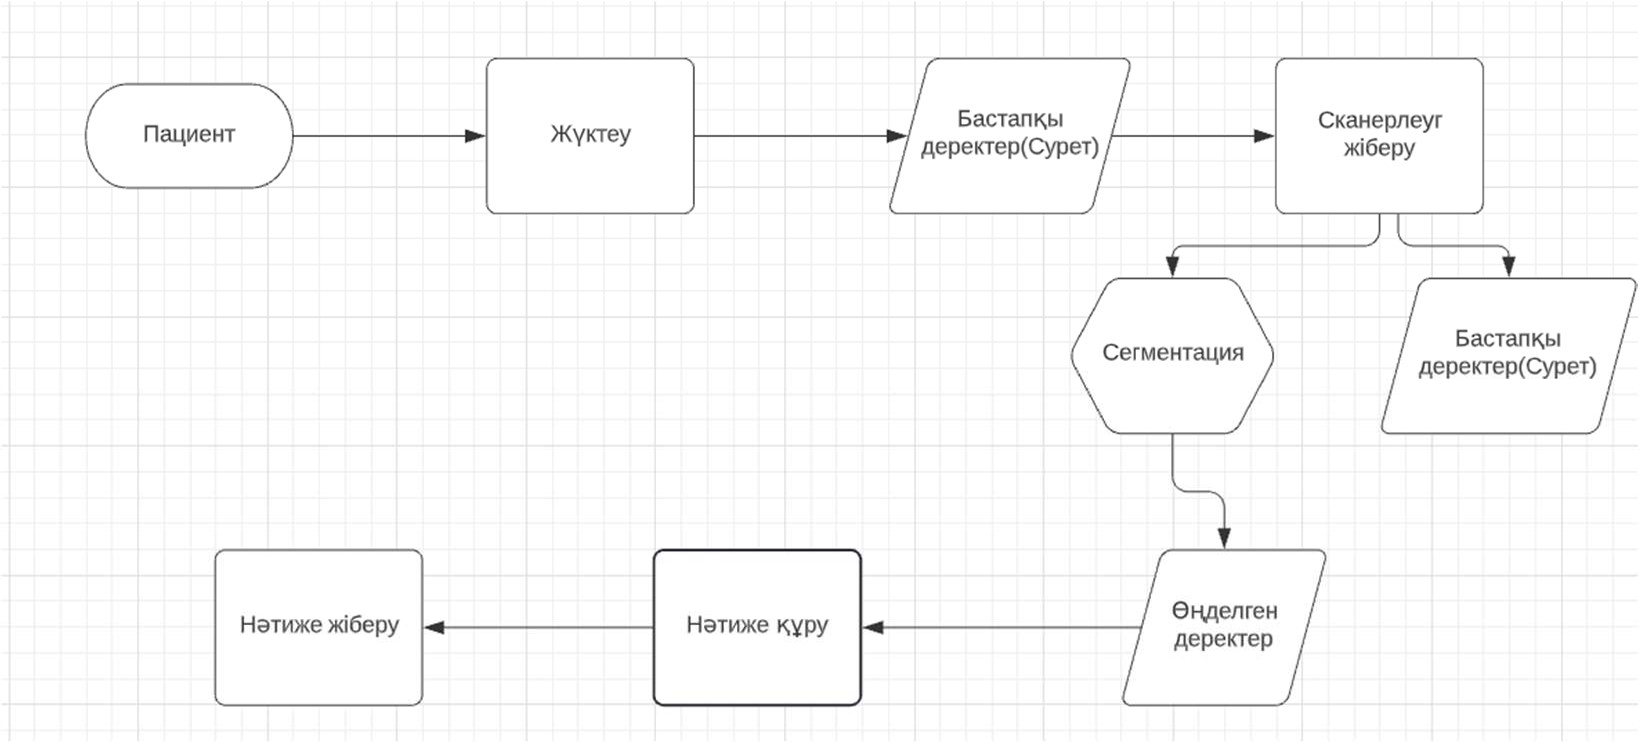
\includegraphics[width=1\textwidth]{assets/191}
	\caption*{\bfseries 1-сурет. Графикалық деректердің жүру картасы}
\end{figure}


\begin{multicols}{2}

Деректер қорының негізгі кестелері бұл «қолданушылар» кестесі және де
өңдеуге арналған «деректер» кестесі болып табылады. Әр «қолданушы»
кестесіне арналған мәнге белгіле бір әдістер ие. Атап өтсек, бұл:
GetImage (); SetImage(); GetResult(); Download(). Төменде, 2-суретте
дизайн деңгейінде жүйені ұсынудың нұсқасы көрсетілген:
\end{multicols}

\begin{figure}[H]
	\centering
	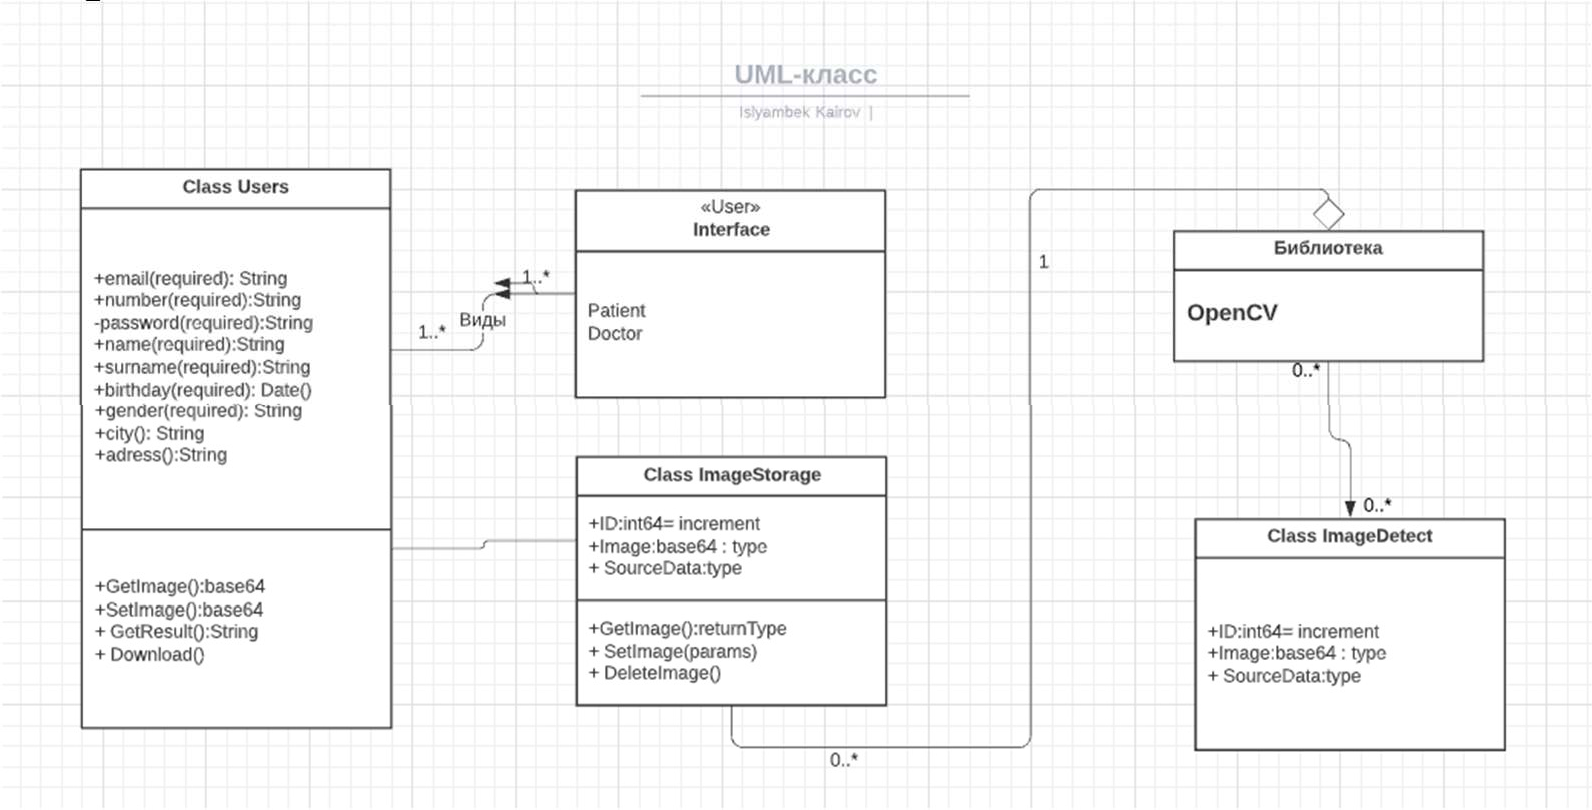
\includegraphics[width=1\textwidth]{assets/192}
	\caption*{\bfseries 2-сурет. Қолданушы және оған қатысты әдістердің мәндері}
\end{figure}


\begin{multicols}{2}

Жүйе келесі негізгі функционалдық блоктардан тұрады: тіркеу,
аутентификация және авторизация, пайдаланушы үшін функционалдылық,
функционал дәрігер, кескін сегментациясының функционалдығы, бетті тану
кітапханасымен біріктіру функционалдығы, сканерлеу нәтижелері.

Жүйені іске асыру үшін келесі технологиялық стек ұсынылады.

Бэкенд: Язык NestJS, NodeJS, БД PostgreSQL.

Серверлік бөлім: Python, OpenCV, numpy.

Фронтенд: ReactNative, TypeScript.

Компьютерлік көруді жіктеудің жалпы проблемасы екі санатты (оқу деректер
жинағы мен сынақ деректер жинағы) ажырату болып табылады. Әдетте
компьютерлік көру тапсырмасы үшін істердің үлкен үлгісі пайдаланылды,
бірақ бұл оқу үшін біздің деректер жинағы шамамен екіге бөлінген 59
кескіннен тұрады, оның 29-ы сынақ үшін және 30-ы оқыту үшін. Деректер
Ұлттық денсаулық институттары {[}10{]} мақалаларынан жарияланған
медициналық суреттер онлайн OpenI репозиторийден алынған. Медицинадағы
цифрлық бейнелеу және коммуникациялар (DICOM) кескінді өңдеу үшін
кескіндерді импорттау, сандық форматқа түрлендіру үшін PyDicom Python
кітапханасы пайдаланылды. Caffe тәрізді басқа платформалармен пайдалану
алдында DICOM файлдарын PNG немесе Joint Photographic Experts Group
(JPEG) пішіміне түрлендіру мүмкін.

Tensorflow, Keras және Google Collab арқылы жүйесінде жазу кітапшалары
ұяшықтарға бөлінген және әрбір ұяшық өз бетінше жұмыс істей алады.
Блокнотта Keras кітапханасынан талаптары жүктелді {[}11{]}. Содан кейін
суреттер туралы ақпарат енгізілді. Соңында, дәуірлер санын (жаттығу
деректері арқылы өту саны) және партия өлшемін (бір уақытта өңделген
кескіндер саны) анықталды. Мембраналық мәліметтер жиынтығы (3-сурет):
\end{multicols}

\begin{figure}[H]
	\centering
	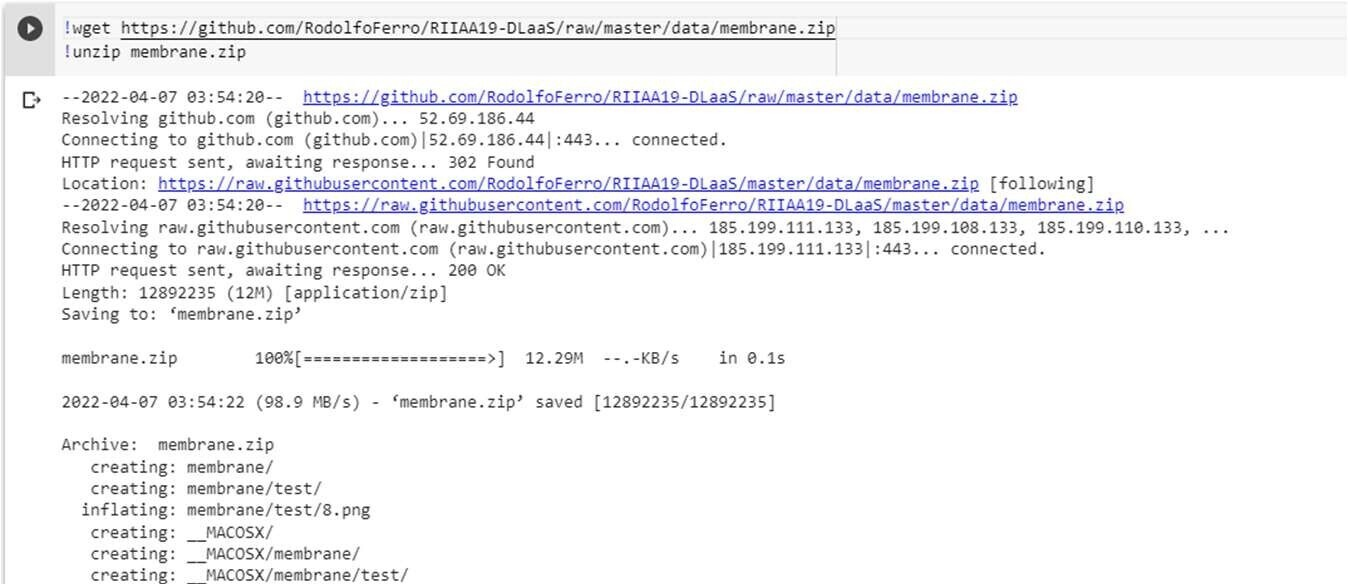
\includegraphics[width=1\textwidth]{assets/193}
	\caption*{\bfseries 3-сурет. Мембраналық мәліметтер жиынтығы}
\end{figure}

\begin{multicols}{2}


Жүйенің модельдеу және жобалау функционал-дығы толықтай зерттелді.

{\bfseries Нәтижелер мен талқылау.} Әзірленген қосымшаның негізгі
технологиясы -- жалпақ кескіндерді тану технологиясы болып табылады. Бұл
технология үшін әртүрлі кітапханалар бар. 4-суретте OpenCV кітапханасы
арқылы жасалған медициналық суреттің сегментация үлгісі көрсетілген.
\end{multicols}

\begin{figure}[H]
  \centering
  \begin{minipage}{0.45\textwidth}
      \centering
      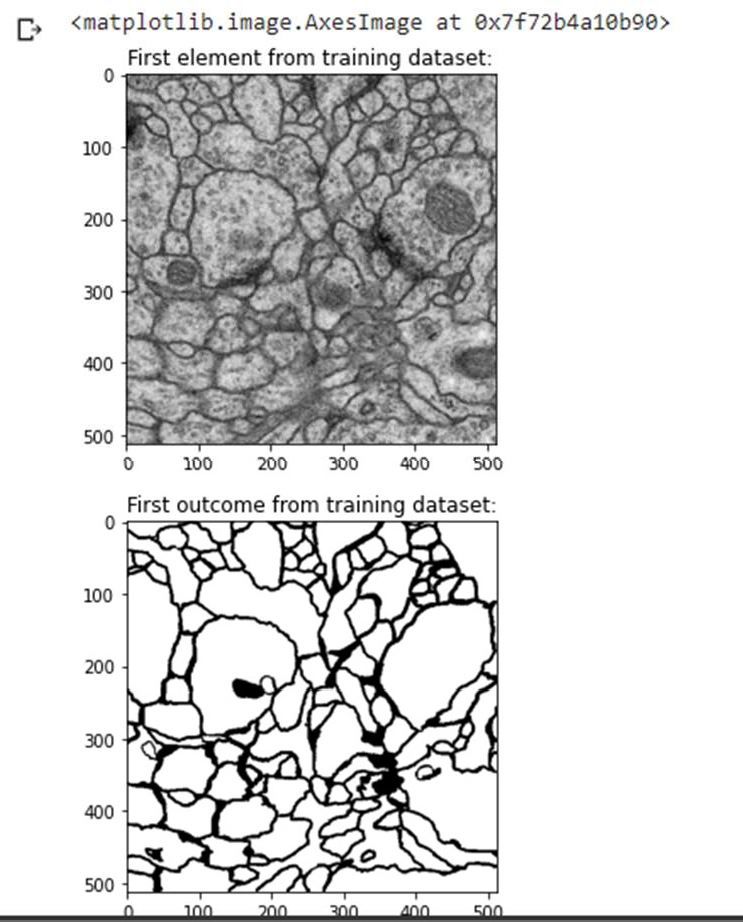
\includegraphics[width=1\textwidth]{assets/194}
      \caption*{}
  \end{minipage}
  \hfill
  \begin{minipage}{0.45\textwidth}
      \centering
      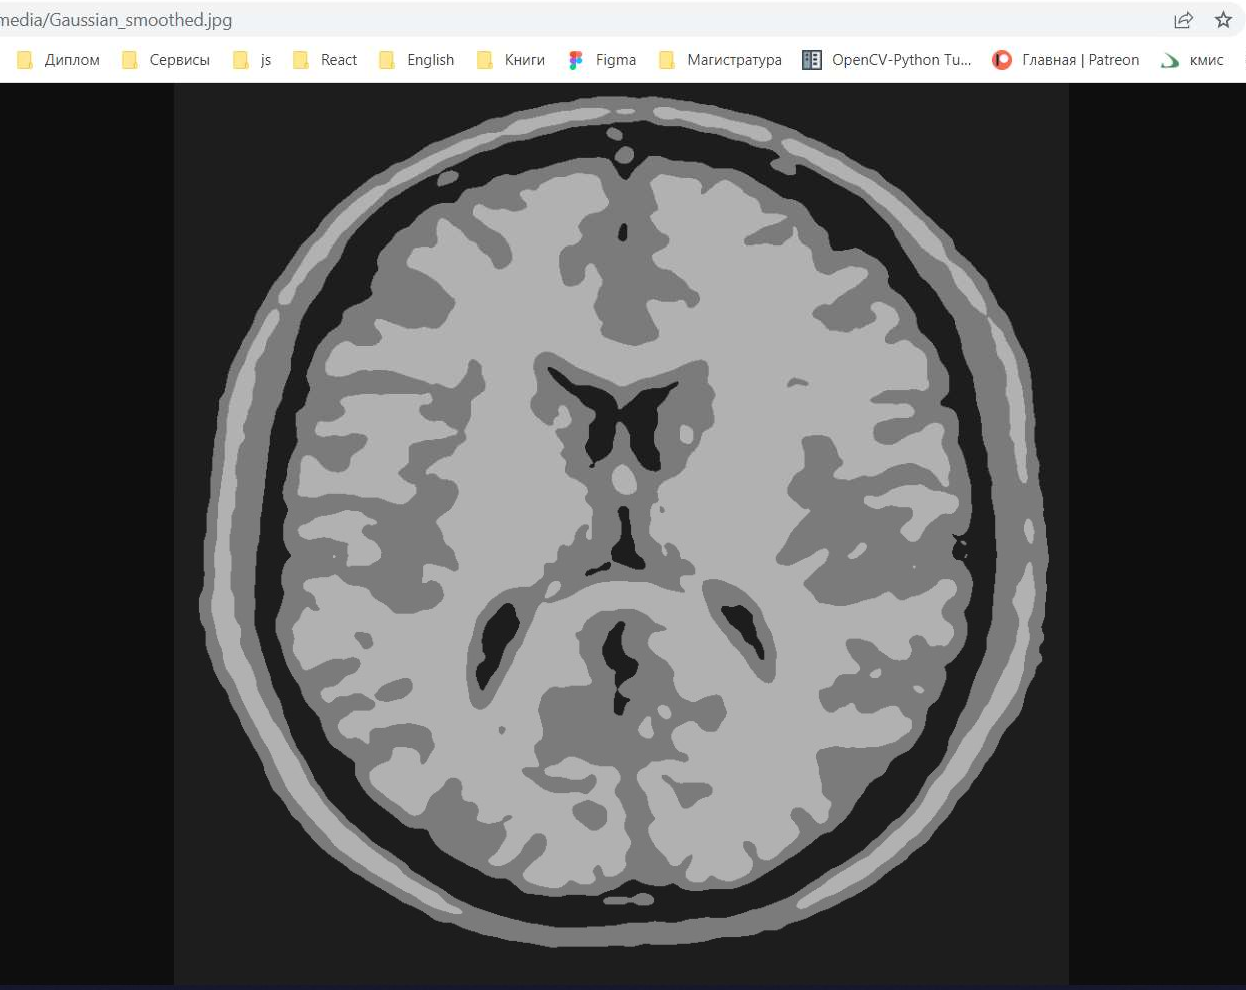
\includegraphics[width=1\textwidth]{assets/195}
      \caption*{}
  \end{minipage}

  \caption*{\bfseries4-сурет. Cегментация үлгісі}
\end{figure}

\begin{multicols}{2}


Бұл зерттеуде серверлік бөлім ретінде Nest js программалық тілі
таңдалды. Сервер алдыңғы бөлігімен өзара әрекеттеседі, веб-параққа ұсыну
үшін деректерді береді және алады. Postman -- бұл басқалар жасаған
RESTful API-ді талдауға немесе өзіңіз жасаған API-ді тексеруге тырысудың
құралы (5-сурет). Тек маршрутты мекен-жай жолына қосу керек, сол жақтағы
ашылмалы тізімнен жауап алу әдісін таңдап, API кілтін «тақырыптар»
бөліміне енгізіп, «әдемі» JSON форматы шығады.

Осы зерттеуде PostgreSQL ДҚБЖ пайдаланыл-ды. Келесі 6-суретте деректер
қорының негізгі кестелері сипатталған.
\end{multicols}

\begin{figure}[H]
	\centering
	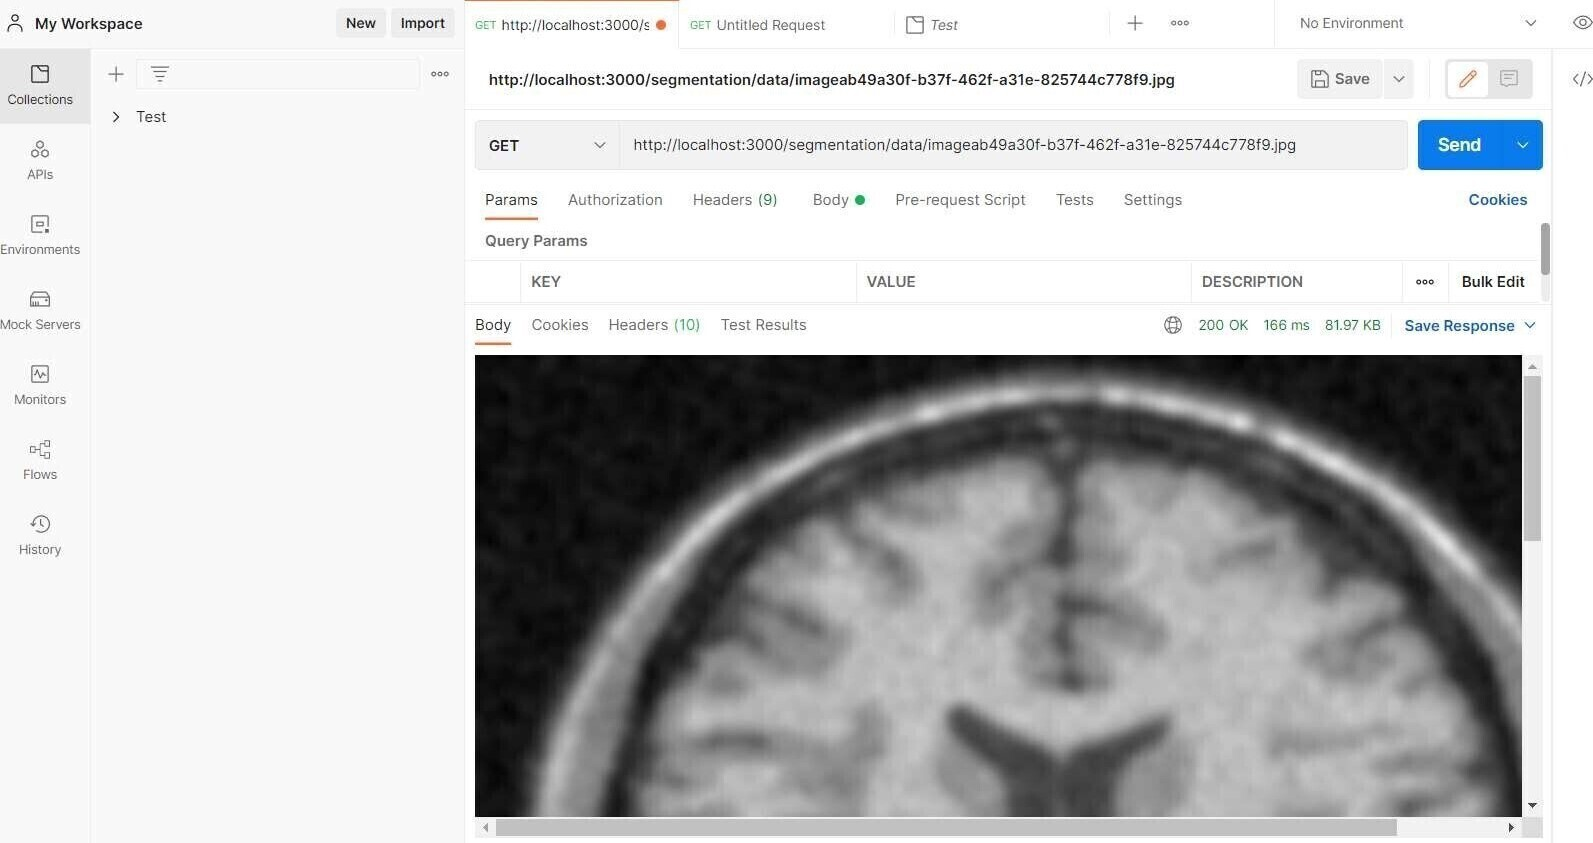
\includegraphics[width=1\textwidth]{assets/196}
	\caption*{\bfseries 5-сурет. Postman арқылы серверді тестілеу}
\end{figure}





\begin{figure}[H]
	\centering
	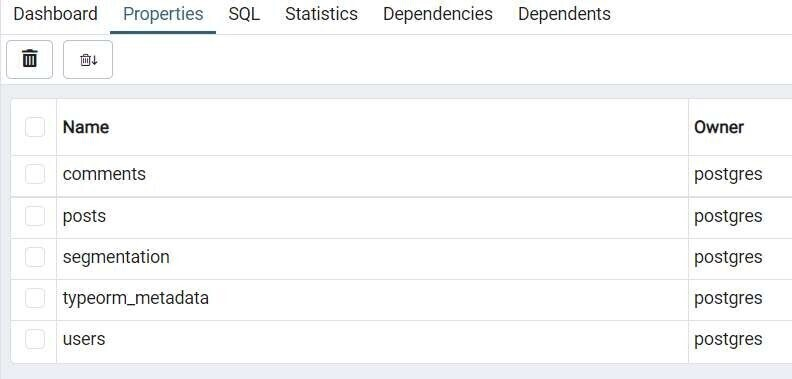
\includegraphics[width=0.6\textwidth]{assets/197}
	\caption*{\bfseries 6-сурет. Деректер қорының негізгі кестелері}
\end{figure}

\begin{multicols}{2}


Клиенттік бөлім React Native Javascript кітапханасы технологиясы арқылы
жүзеге асырылған. Одан басқа мобильді қосымша құру кезінде келесі
қосымша кітапханалар орнатылды: Axios, Buffer,
@react-native-picker/picker, FontAwesome5,
@react-native-async-storage/async-storage, react-native-gesture-handler,
formik, @react-navigation/bottom-tabs, @react-navigation/stack,
@react-navigation/native. Қосымшаның демо нұсқасы Аndroid studio
программалық қамтама арқылы құрастырылады (7-сурет).
\end{multicols}

\begin{figure}[H]
	\centering
	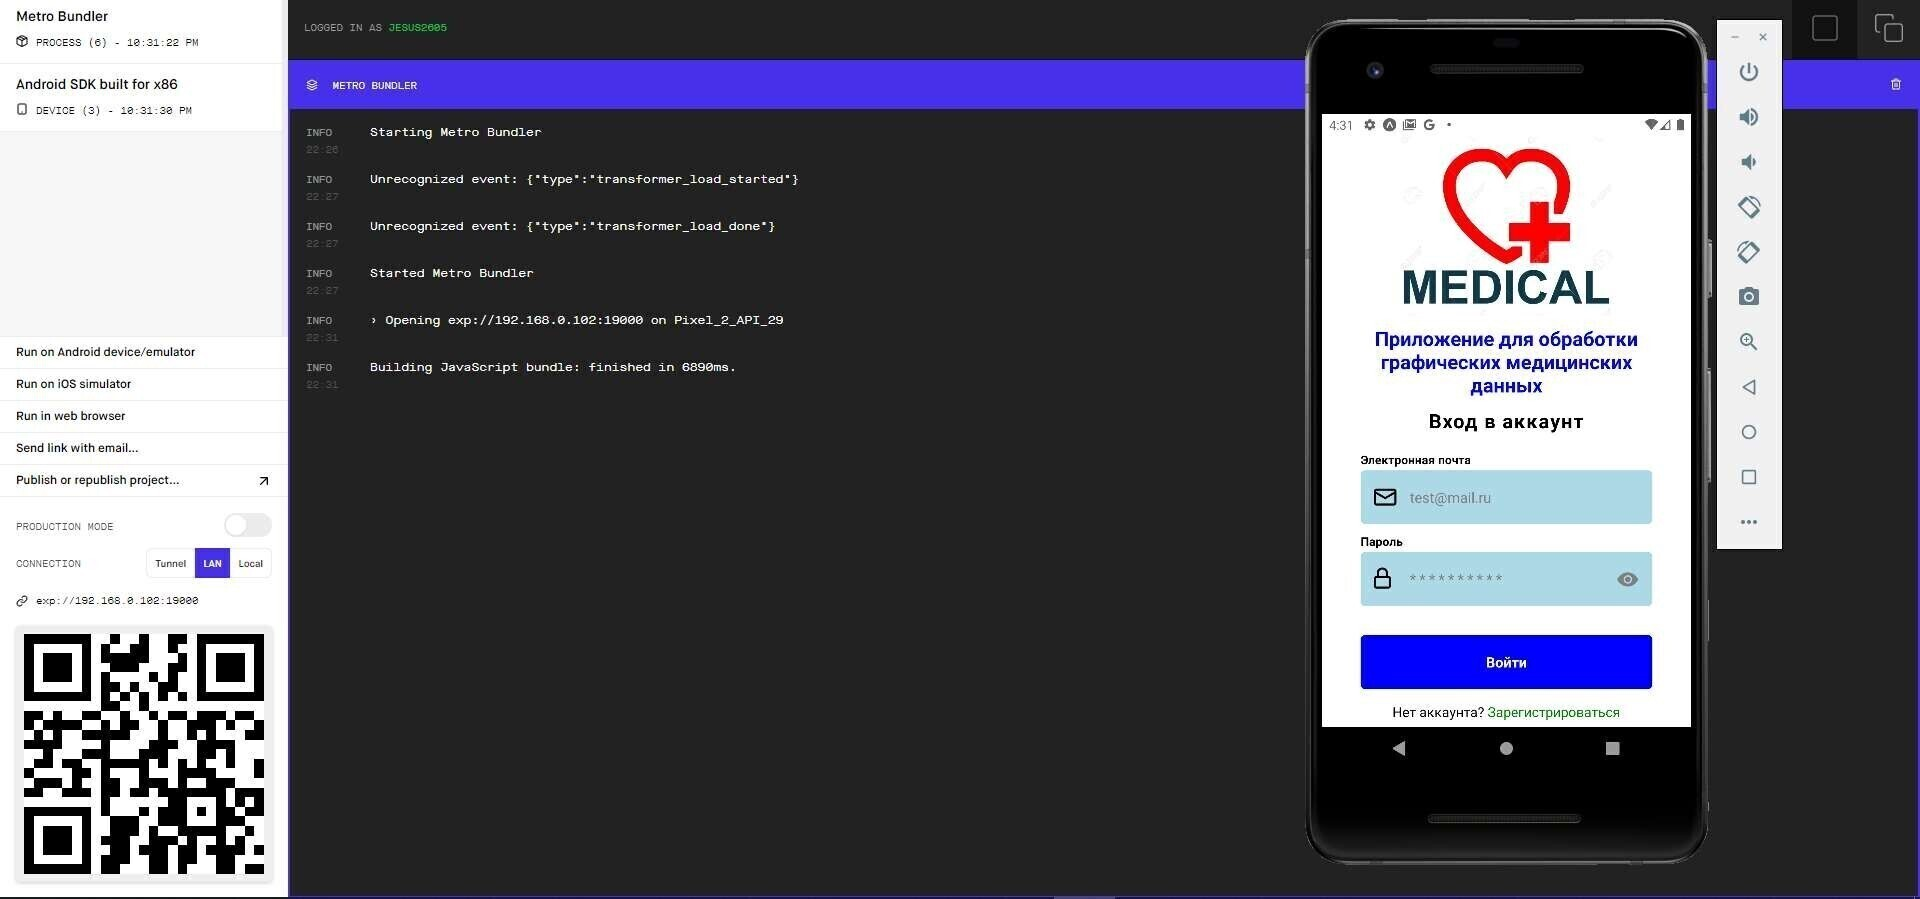
\includegraphics[width=0.8\textwidth]{assets/198}
	\caption*{\bfseries 7-сурет. Аndroid studio ортасында қосымшаның интерфейсі}
\end{figure}

\begin{multicols}{2}


Жобаңың package.json файлы -- бұл қосымшамен өзара әрекеттесуде.
Виртуалды DOM тұжырымдамасы беретін абстракция дәрежесінің арқасында
React Native «көпір» жазуға тура келгенше басқа платформаларға назар
аудара алады.

{\bfseries Қорытынды.} Зерттеу жүргізу барысында программалық қосымша
арқылы медициналық кескіндерді сегментациялау жүзеге асырылды.
Медициналық кескіндерді сегментациялау әдістері зерттелінді. Әдістерді
толықтай талдап, артықшылықтары мен кемшіліктері анықталды. Әзірленген
жүйенің жобалау және модельдеуі сипатталды. Техникалық тапсырма кезінде
пайдаланушы, дәрігер және әкімші деген үш пайдаланушы түрі анықталды. Әр
пайдаланушы түріне бөлек функционал сипатталып, жасалынды. Жобада
қолданылған әр технология зерттелді. Практикада қолданылған келесі
технологиялар: Серверлік бөлім -- NestJS; Клиенттік бөлім --
ReactNative; Компьютерлік көру модулі -- OpenCV; Дерекқор базасы --
PostgresSQL. Программалық қамтамасыздандыру құру кезінде келесі
лицензияланған программаларды қолдандық: Visual Studio Code; Postman;
TablePlus; pgAdmin; ExpoGo. Осылайша, сегменттелген кескіндер
диагностиканың дәлдігін жақсартады, оларды пайдалануда, сақтауда және
одан әрі түсіндіруде ресурстарды үнемдейді. Мұндай қосымшалар үйден
шықпай-ақ бірнеше дәрігерден кеңес алуға мүмкіндік береді. Осы жерде
және қазір суретті оқудағы дәлдікті жақсартуға мүмкіндік беретін мұндай
қосымшаның Қазақстанда жұмыс істеуі басқа клиникалық тексеру әдістерімен
бірге орасан зор жетістік болуы мүмкін, өйткені ол дәрігер мен
пациенттің ортақ пікіріне жетуіне көмектеседі, нақты қорытынды жасалып,
кейіннен диагноз қойылады. Сондай-ақ, қолданбалы бұлтқа зерттеулердің
біраз көлемін сақтауға мүмкіндік беретін дерекқор базасы жасалынды және
кроссплатформалы қосымша құрылды. Құрылған мобильді қосымшаға толықтай
тестілеу жүргізілді. Қазақстандағы медицина саласында сәулелік
бейнелерді сегментациялау пациент диагнозын неғұрлым дәл диагностикалау
мен одан әрі верификациялау ең қажетті функцияларға айналуы мүмкін,
демек, әртүрлі ауруларды уақтылы анықтаудың арқасында халықтың өмір сүру
сапасын жақсартатын неғұрлым ұтымды және мақсатты емдеуге кең
қолданысына ие болады.
\end{multicols}

\begin{center}
  {\bfseries Әдебиеттер}
  \end{center}


  \begin{noparindent}

\begin{enumerate}
\def\labelenumi{\arabic{enumi}.}
\item
  Mei, H., Xu, K., Zhou, Y.~et al.~Camouflaged Object Segmentation with
  Omni Perception.~Int J Comput Vis. -2023. -Vol. 131. - P.3019-3034.
  https://doi.org/10.1007/s11263-023-01838-2
\item
  Маркелов, К. С. Модель повышения информативности цифровых изображений
  на базе метода суперразрешения / К.С. Маркелов // Инженерный вестники
  -- М. : ФГБОУ ВПО «МГТУ им. Н.Э. Баумана». -- 2013. -- Вып.3. -- С.
  525--542.
\item
  OpenCV tutorial. URL.
  https://medium.com/analytics-vidhya/opencv-tutorial-introduction-and-image-\\basics-7675866eb95a(өтініш
  берген күні: 9.03.2024)
\item
  Clarke LP, Velthuizen RP, Camacho MA, Heine JJ, Vaidyanathan M, Hall
  LO, Thatcher RW, Silbiger ML. MRI segmentation: methods and
  applications. Magn Reson Imaging.-1995. -Vol. 13(3). -P.343-368. doi:
  10.1016/0730-725x(94)00124-l. PMID: 7791545.
\item
  Chaohui Wang, Nikos Komodakis, Nikos Paragios. Markov Random Field
  modeling, inference \& learning in computer vision \& image
  understanding//A survey, Computer Vision and Image Understanding.
  -2013. -Vol. 117. Iss. 11. -P. 1610-1627.
  https://doi.org/10.1016/j.cviu.2013.07.004.
\item
  Modernizing Computer Vision with the Help of Neural Networks.
  {[}URL{]}. - https://marutitech.com/\\computer-vision-neural-networks/
  (өтініш берген күні: 9.03.2024)
\item
  Шуйтенов, Г., У.~Турусбекова, М.~Муратбеков Анализ научных текстов на
  основе языковых моделей алгоритмами распределенной обработки// Вестник
  КазУТБ -2023. -№4(21). doi:10.58805/kazutb.\\v.4.21-220.
\item
  McInerney T, Terzopoulos D. Deformable models in medical image
  analysis: a survey. Published in Medical Image Analysis. -1996.
  -Vol.1(2). -P. 91-108.
  https://web.cs.ucla.edu/\textasciitilde dt/papers/mia96/\\mia96.pdf
\item
  An end-to-end platform for machine learning: Get started with
  TensorFlow https://www.tensorflow.org/\\?hl=ru (өтініш берген күні:
  12.03.2024)
\item
  Open Access Biomedical Image Search Engine. https://openi.nlm.nih.gov.
  \\(өтініш берген күні: 15.03.2024)
\item
  Декодирование файлов DICOM для получения медицинских изображений.
 \\ https://www.tensorflow.org/io/tutorials/dicom (өтініш берген күні:
  15.03.2024)
\end{enumerate}
\end{noparindent}


\begin{center}
  {\bfseries References}
  \end{center}

\begin{noparindent}

1. Mei, H., Xu, K., Zhou, Y. et al. Camouflaged Object Segmentation with
Omni Perception. Int J Comput Vis. -2023. -Vol. 131. - P.3019-3034.
https://doi.org/10.1007/s11263-023-01838-2

2. Markelov, K. S. Model\textquotesingle{} povyshenija informativnosti
cifrovyh izobrazhenij na baze metoda superrazreshe-nija / K.S. Markelov
// Inzhenernyj vestniki -- M. : FGBOU VPO «MGTU im. N.Je. Baumana». --
2013. -- Vyp.3. -- S. 525--542. {[}in Russian{]}

3. OpenCV tutorial. URL.
https://medium.com/analytics-vidhya/opencv-tutorial-introduction-and-image-basics-7675866eb95a(date
of application: 9.03.2024)

4. Clarke LP, Velthuizen RP, Camacho MA, Heine JJ, Vaidyanathan M, Hall
LO, Thatcher RW, Silbiger ML. MRI segmentation: methods and
applications. Magn Reson Imaging.-1995. -Vol. 13(3). -P.343-368. doi:
10.1016/0730-725x(94)00124-l. PMID: 7791545.

5. Chaohui Wang, Nikos Komodakis, Nikos Paragios. Markov Random Field
modeling, inference \& learning in computer vision \& image
understanding//A survey, Computer Vision and Image Understanding. -2013.
-Vol. 117. Iss. 11. -P. 1610-1627.
https://doi.org/10.1016/j.cviu.2013.07.004.

6. Modernizing Computer Vision with the Help of Neural Networks.
{[}URL{]}. - https://marutitech.com/\\computer-vision-neural-networks/
(date of application: 9.03.2024)

7. Shujtenov, G., U. Turusbekova, M. Muratbekov Analiz nauchnyh tekstov
na osnove jazykovyh modelej algoritmami raspredelennoj obrabotki//
Vestnik KazUTB -2023. -№4(21). doi:10.58805/kazutb.v.4.21-220. {[}in
Russian{]}

8. McInerney T, Terzopoulos D. Deformable models in medical image
analysis: a survey. Published in Medical Image Analysis. -1996.
-Vol.1(2). -P. 91-108.
https://web.cs.ucla.edu/\textasciitilde dt/papers/mia96/mia96.pdf

9. An end-to-end platform for machine learning: Get started with
TensorFlow https://www.tensorflow.org/\\?hl=ru (date of application:
12.03.2024)

10. Open Access Biomedical Image Search Engine.
\\https://openi.nlm.nih.gov. (date of application: 15.03.2024)

11. Dekodirovanie fajlov DICOM dlja poluchenija medicinskih
izobrazhenij. \\https://www.tensorflow.org/io/tutorials/dicom (date of
application: 15.03.2024)
\end{noparindent}


\emph{{\bfseries Авторлар туралы мәліметтер}}
\begin{noparindent}

Есенгалиева Ж.С. - PhD, доцент м.а., Л.Н. Гумилев атындағы Еуразия
ұлттық университеті, Астана, Қазақстан,е-mail:jannayess@gmail.com;

Оралбекова Ж.О. - PhD, доцент, Л.Н. Гумилев атындағы Еуразия ұлттық
университеті, Астана, Қазақстан, е-mail:oralbekova@bk.ru;

Турарова М.К. - PhD, Л.Н. Гумилев атындағы Еуразия ұлттық университеті,
Астана, Қазақстан,

е-mail:marzhan\_08@mail.ru
\end{noparindent}

\emph{{\bfseries Information about the authors}}
\begin{noparindent}

Yessengaliyeva Zh.S. - PhD, аcting associate professor, Eurasian
national university, Astana, Kazakhstan,

е-mail:jannayess@gmail.com;

Oralbekova Zh.O. - PhD, associate professor, Eurasian national
university, Astana, Kazakhstan,

е-mail:oralbekova@bk.ru;

Turarova M.K. - PhD, Eurasian national university, Astana, Kazakhstan,
е-mail:marzhan\_08@mail.ru
\end{noparindent}


